
The project was made using the python 3 language and it also involved programming a GUI so that the user can develop their graphs and see how the algorithm works, step by step. To see the functioning project, one external library PyQt5 is needed. After that is installed, the project can be run by running the file GUI.py. We have included few sample graph snapshots below:
    \begin{figure}[h]
     \centering
     \begin{subfigure}{}
        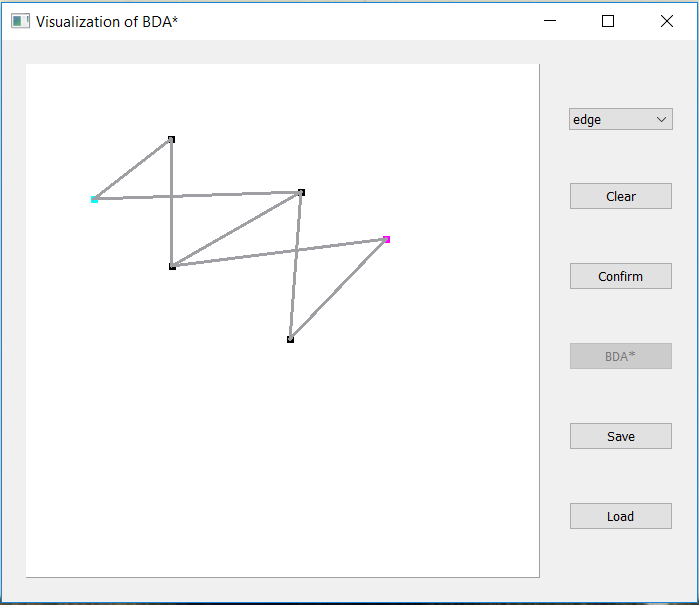
\includegraphics[width=0.4\textwidth]{bda.JPG}
        \caption{Sample Graph 1}
        \label{fig:1}
     \end{subfigure}
     \begin{subfigure}{}
        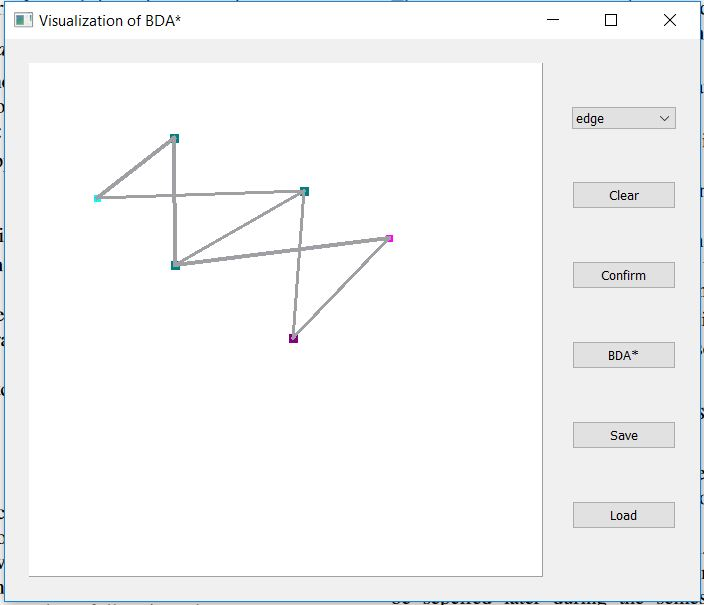
\includegraphics[width=0.4\textwidth]{bda2.JPG}
        \caption{Sample Graph output}
        \label{fig:1}
        \end{subfigure}
     \end{figure}

\pagebreak
\begin{itemize}
    \item By analyzing different types of graphs we see that the algorithm does not always give you the shortest path. There may be cases in which the two path: one from source and other from the goal node don't meet till at nay node except the terminal nodes. 
    \item The code for the project can be found in the zip file with the report. 
\end{itemize}


